% This is the master file of the folder structure.

% First, the preamble needs to be called. This contains all the 'under the hood' stuff for your document.
% Use \input rather than than \include for .tex files, because \input can be nested and don't include a page break.
% This file contains your LaTeX preamble. A preamble is a part of your document where all required packages and macros can be defined. This needs to be done before the \begin{document} command.

% Documentclass:
% Standard LaTeX classes are: article, book, report, slides, and letter. These cover the basis, but are not best. More advanced users might want to try out the KOMA classes or the memoir class. Optional arguments: 10pt. The font size of the main content is set to 10pt with the option between [].
\documentclass{llncs}
\usepackage[utf8]{inputenc}

% Geometry:
% The papersize of the document is defined with the geometry package. Here, the size is set to A4 with a4paper. Other possibilities are a5paper, b5paper, letterpaper, legalpaper and executivepaper.
\usepackage[a4paper]{geometry}

% AMS math packages:
% Required for proper math display.
%\usepackage{amsmath,amsfonts,amsthm}	% conflict with the llncs package
\usepackage{amsmath,amsfonts}			% to avoid conflict with the llncs package
%\usepackage{amsfont} create a conflict so it's not used
\usepackage{amssymb}
\usepackage{mathtools}
% For case equation with nested label
% \usepackage{cases} NOT USEFUL



% Graphicx:
% If you want to include graphics in your document, the graphicx package is required.
\usepackage{graphicx}

% Graphic path declaration:
\graphicspath{{figs/}}

% Tabu:
% To test if this package could be the latest package for my work
\usepackage{tabu}

% [OLD] Booktabs:
% The booktabs package is needed for better looking tables. 
\usepackage{booktabs}

% [OLD] Tables:
\usepackage[table]{xcolor}
\usepackage{multirow}
%\usepackage{tabularx}

\newcommand{\win}{\cellcolor[gray]{0.9}}

% Enumeration:
% To manipulate the listing of object
\usepackage[inline]{enumitem}
\setlist*[enumerate,1]{%
	label=(\roman*),
}
% [Alternative]
%\usepackage{easylist}

% SIunitx:
% The SIunitx package enables the \SI{}{} command. It provides an easy way of working with (SI) units.
\usepackage{siunitx}

% URL:
% Clickable URL's can be made with this package: \url{}.
%\usepackage{url}

% Caption:
% For better looking captions. See caption documentation on how to change the format of the captions.
%\usepackage{caption}

% Hyperref:
% This package makes all references within your document clickable. By default, these references will become boxed and colored. This is turned back to normal with the \hypersetup command below.
\usepackage{hyperref}
\hypersetup{colorlinks=false,pdfborder=0 0 0}

% Cleveref:
% This package automatically detects the type of reference (equation, table, etc.) when the \cref{} command is used. It then adds a word in front of the reference, i.e. Fig. in front of a reference to a figure. With the \crefname{}{}{} command, these words may be changed.
\usepackage{cleveref}
\crefname{equation}{equation}{equations}
\crefname{figure}{figure}{figures}	
\crefname{table}{table}{tables}

% Pseudo code packages:
\usepackage[ruled,linesnumbered]{algorithm2e}
\usepackage{algorithmicx}
\usepackage{algpseudocode}

% Verbatim:
% Typewriter formatting and comment environment
\usepackage{verbatim}

% Bibliography style
%\usepackage{natbib}



% Command

% For the level structure depending of the 

% The title page is created with the command \maketitle which needs to be placed after the \begin{document} command. To create the titlepage, some entries are needed: the name of the autor is defined by \author{}, the title by the entry \title{} and the date by the command \date{}. Note that the current date is displayed with \today.

\title[ACS Scheduling]{
Ant colony system for scheduling problem
} % The short title appears at the bottom of every slide, the full title is only on the title page

\author[Ambrosini \and Nicol\`{o}]{Ambrosini,~Luca \and Nicol\`{o},~Giancarlo %\and Miguel~A.~Salido \and Adriana~Giret \and Federico~Barber
} % Your name
\institute[UPV] % Your institution as it will appear on the bottom of every slide, may be shorthand to save space
{
	\inst{1}%
	Universitat Polit\`{e}cnica de Val\`{e}ncia % Your institution for the title page
	%\and
	%\inst{2}%
	%Instituto Universitario de Autom\'{a}tica e Inform\'{a}tica Industrial \\
	%\medskip
	%\textit{giani1@dsic.upv.es, msalido@dsic.upv.es, agiret@dsic.upv.es, fbarber@dsic.upv.es} % Your email address
}

% logo of my university
\titlegraphic{
	%
\includegraphics[width=1cm]{AI2_logo.jpg}\hspace*{4.75cm}~%
	
\includegraphics[width=2cm]{UPV_logo.png}%
}

%\logo{
%	\includegraphics[height=0.8cm]{ICAPS_logo.png}%
%}

%\date{\today} % Date, can be changed to a custom date
\date[May, 8th 2017]{May, 8th 2017 }




% All the actual content of your document should be placed after \begin{document} and before \end{document}. This content should be placed in the docs folder and can then be called with \input{docs/filename}.
\begin{document}

% Here the actual title page is printed, based on the given entries \author{}, \title{} and \date{}.
%\maketitle

% The table of contents can be automatically generated with the \tableofcontents command. Note that you need to compile the document twice in order to see the changes in the table of contents.
%\tableofcontents

% List of figures
%\listoffigures
 
% List of tables
%\listoftables

% The list of algorithm
%\listofalgorithms

% The \input{} command reads and processes the indicated example.tex file. Note that docs/ locates the folder where the .tex file is stored.
%----------------------------------------------------------------------------------------
%	INTRODUCTION SLIDES
%----------------------------------------------------------------------------------------

\begin{frame}
\titlepage % Print the title page as the first slide
\end{frame}


\begin{frame} \frametitle{Overview} % Table of contents slide, comment this block out to remove it
\tableofcontents[hideallsubsections] % Throughout your presentation, if you choose to use \section{} and \subsection{} commands, these will automatically be printed on this slide as an overview of your presentation
%\tableofcontents[currentsection]
\end{frame}

%------------------------------------------------
\section{Introduction}
%------------------------------------------------


\begin{frame} \frametitle{Idea}

\begin{block}{Aim}
	Novel work to tackle literature leaks in the scheduling domain applying meteheuristic approaches.
\end{block}

\medskip
\begin{columns}[c]
	\begin{column}[c]{6cm}
		Scheduling domain:
		\begin{itemize}
			\item Energy aware scheduling
			\item Realistic problem (setup, release, due date)
		\end{itemize}
	\end{column}
	\pause
	\begin{column}[c]{6cm}
		Metaheuristic:
		\begin{itemize}
			\item Ant Colony Optimization
			\item Ant Colony System
		\end{itemize}
	\end{column}
\end{columns}

\end{frame}


\begin{frame} \frametitle{Motivation}
\pause
Why scheduling problem?
\begin{itemize}[<+->]
	\item most of daily life problem can easily map in scheduling problem
	\begin{itemize}
		\item industrial/manufacturing environment 
		\item supply-chain management
		\item space orbit 
	\end{itemize}
	\item optimization of shared resources
	\item search for efficiency and cost reduction
	\item avoid critical situation
\end{itemize}

\begin{columns}[c]
	\begin{column}[c]{6cm}
		\begin{figure}
			\centering
			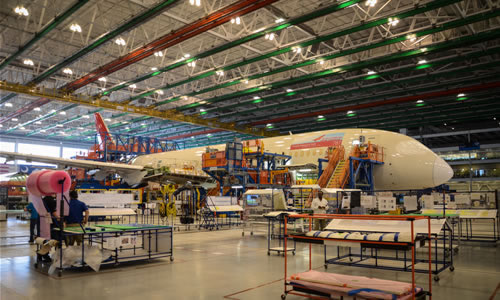
\includegraphics[width=.8\columnwidth]{boeing}
			%\caption{Interaction sequence to solve the distributed scheduling problem}
		\end{figure}
	\end{column}
	\pause
	\begin{column}[c]{6cm}
		\begin{figure}
			\centering
			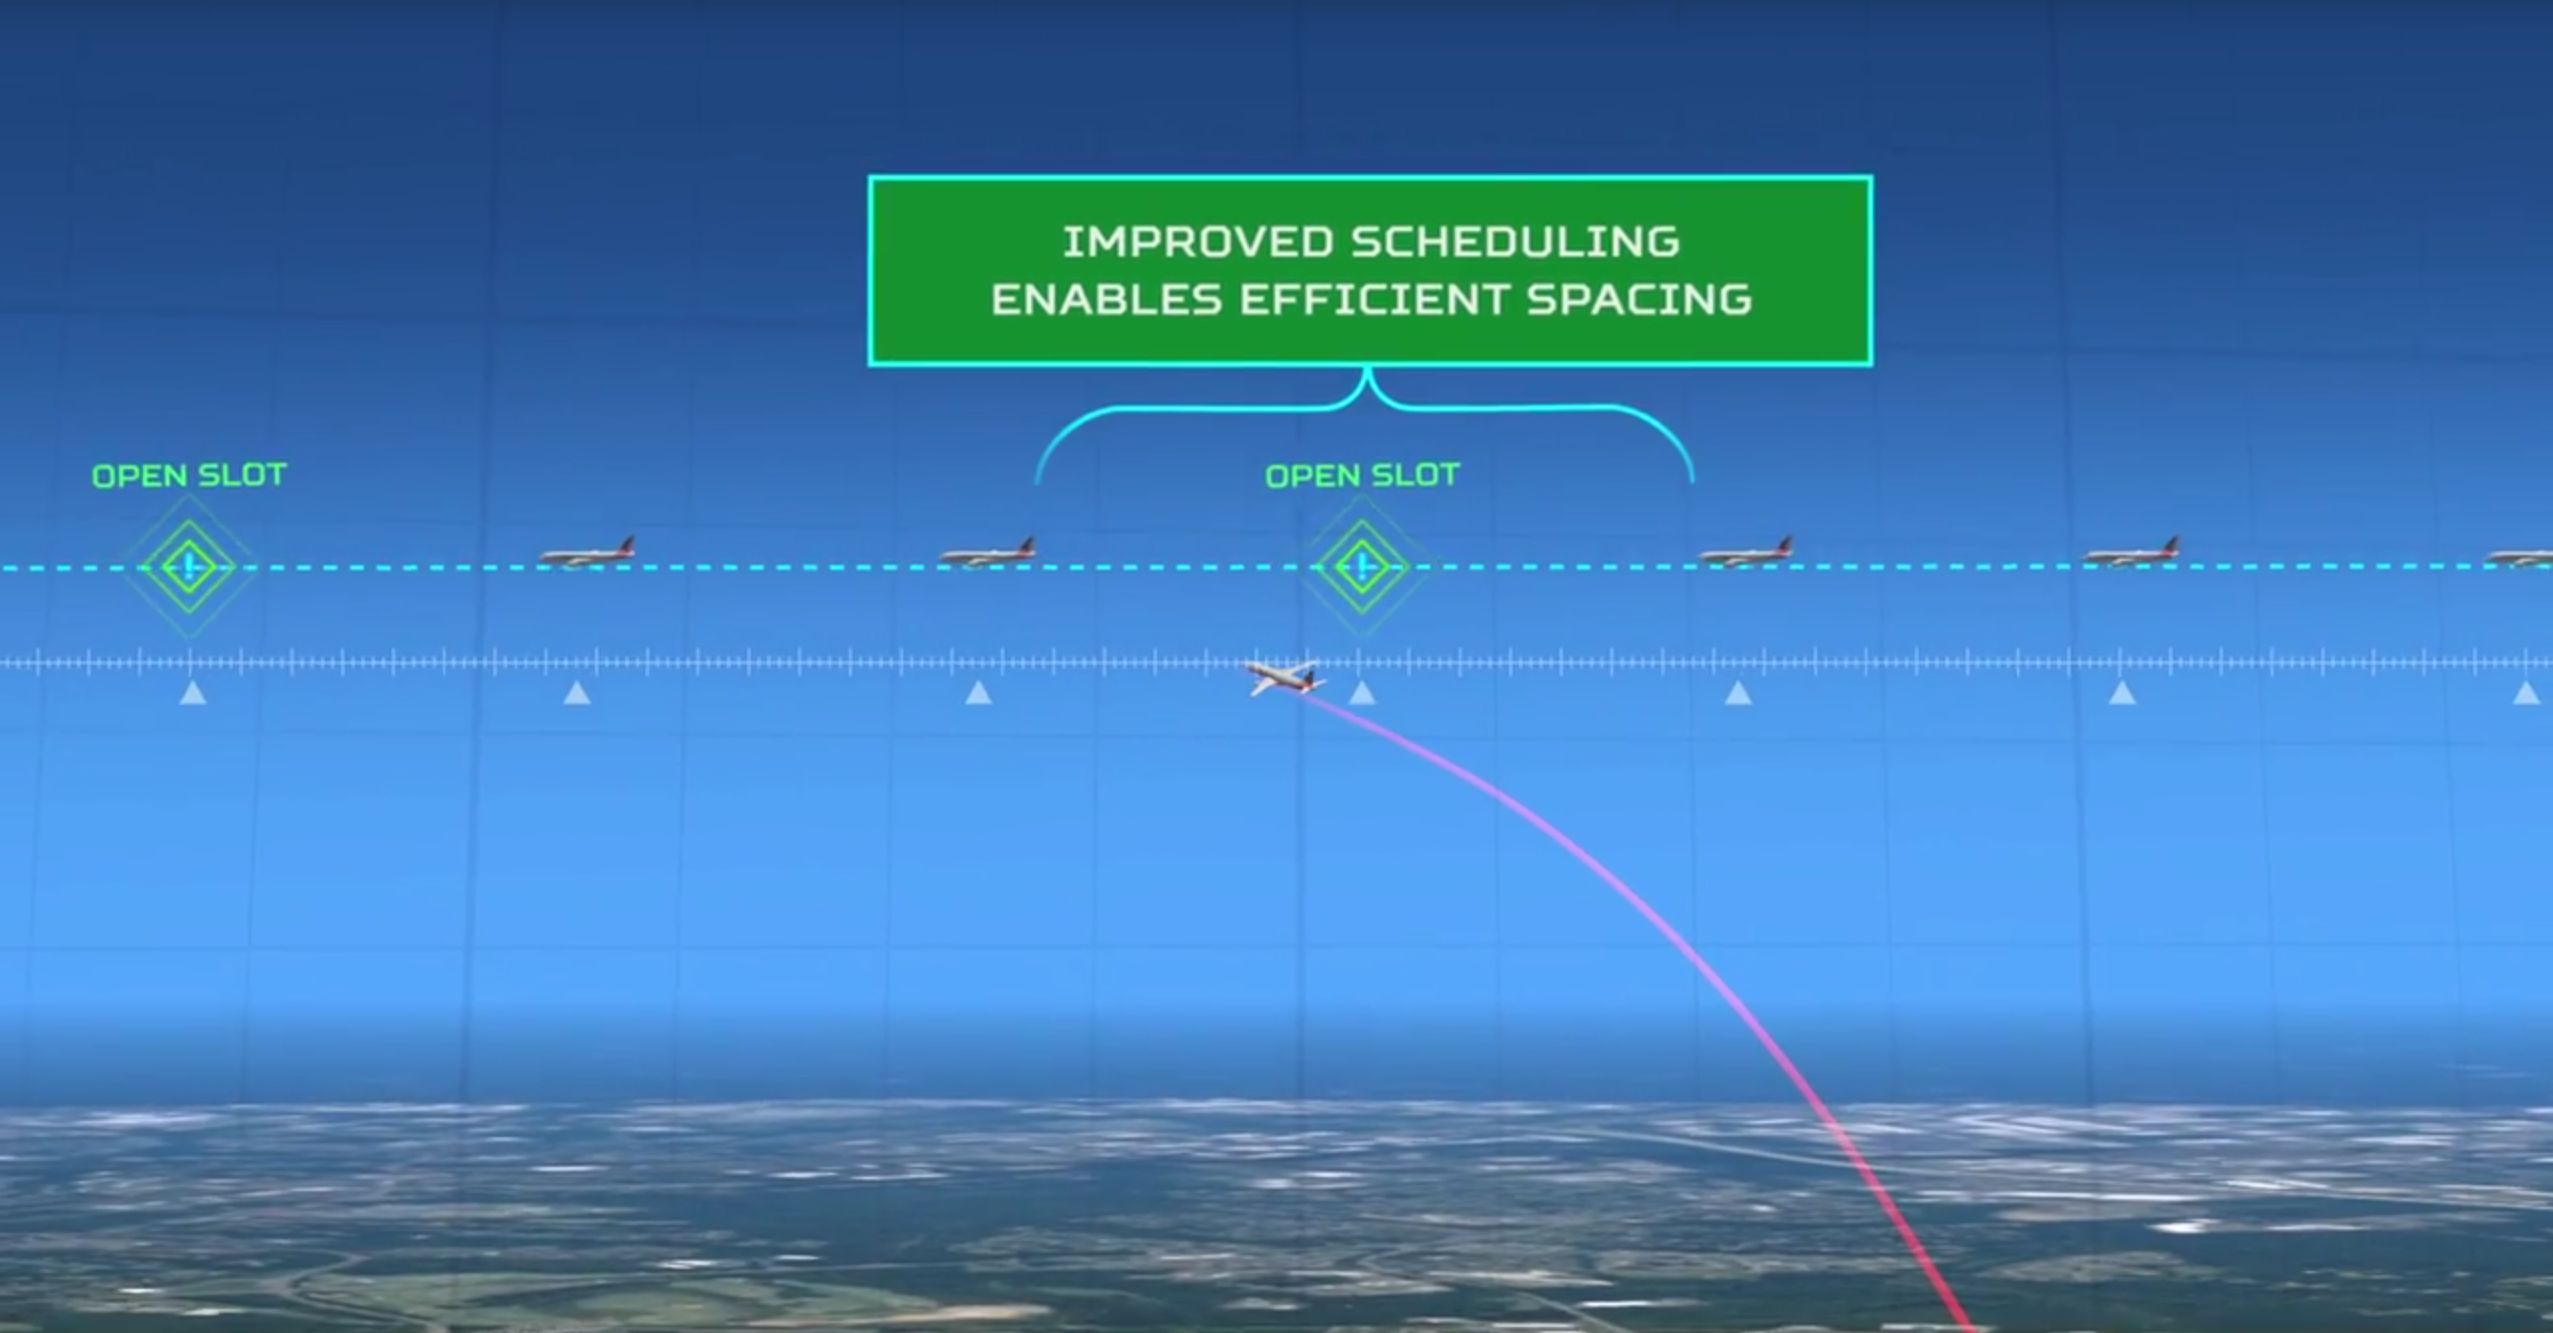
\includegraphics[width=.8\columnwidth]{nasa}
			%\caption{Interaction sequence to solve the distributed scheduling problem}
		\end{figure}
	\end{column}
\end{columns}

\end{frame}			% Intoduction (title, table of contents)
\section{Task Definition} \label{sec:problem}

description of the problem

olitical conversation in Twitter increases when a General Election comes close. Analyzing the topics discussed by users provides interesting insights of this growing public conversation on politics.

In COSET, the aim is to classify a corpus of political tweets in 5 categories of classification: political issues, related to the most abstract electoral confrontation; policy issues, about sectorial policies; personal issues, on the life and activities of the candidates; campaign issues, related with the evolution of the campaign; and other issues.

The tweets are written in Spanish and they talk about the 2015 Spanish General Election. In the training phase participants will be provided with Twitter Ids and their manually issue codification.

We cordially invite all researchers and practitioners from all fields to participate in COSET.

category to differenciate

problem over the tweet (chiedi alla tipa di torino i tweet challenges)		% Problem
%%------------------------------------------------
\section{MIP model}
%------------------------------------------------

\begin{frame} \frametitle{MIP model} 

\begin{itemize}[<+->]
\item use basic functionality of IBM ILOG CPLEX optimization studio
\item comprehende basic constructs of the OPL language
\item apply basic OPL constructs over a constraint satisfaction problem (CSP)
\item comprehende advanced constructs of the OPL language
\item recognize a job-shop scheduling problems
\item apply advanced constructs to model a job-shop scheduling problem
\end{itemize}

\end{frame}			% MIP model
%------------------------------------------------
\section{Ant colony system}
%------------------------------------------------

\begin{frame} \frametitle{Ant colony} 

\begin{itemize}[<+->]
	\item Meta-heuristic proposed by [Colorni, et Al], improved by [Dorigo, Gambardella, et al.]
	\item Mimicry of ants behavior to find optimal path between nest and food
	\begin{itemize}
		\item Transition rules
	\end{itemize}
	\item Indirect communication between ants through pheromones amount
	\begin{itemize}
		\item Update rules
	\end{itemize}
	\item State of the art in various optimization problem
\end{itemize}

\end{frame}


\begin{frame}\frametitle{Ant exaple}
\begin{figure}[t]
	\label{fig:ants}
	\centering
	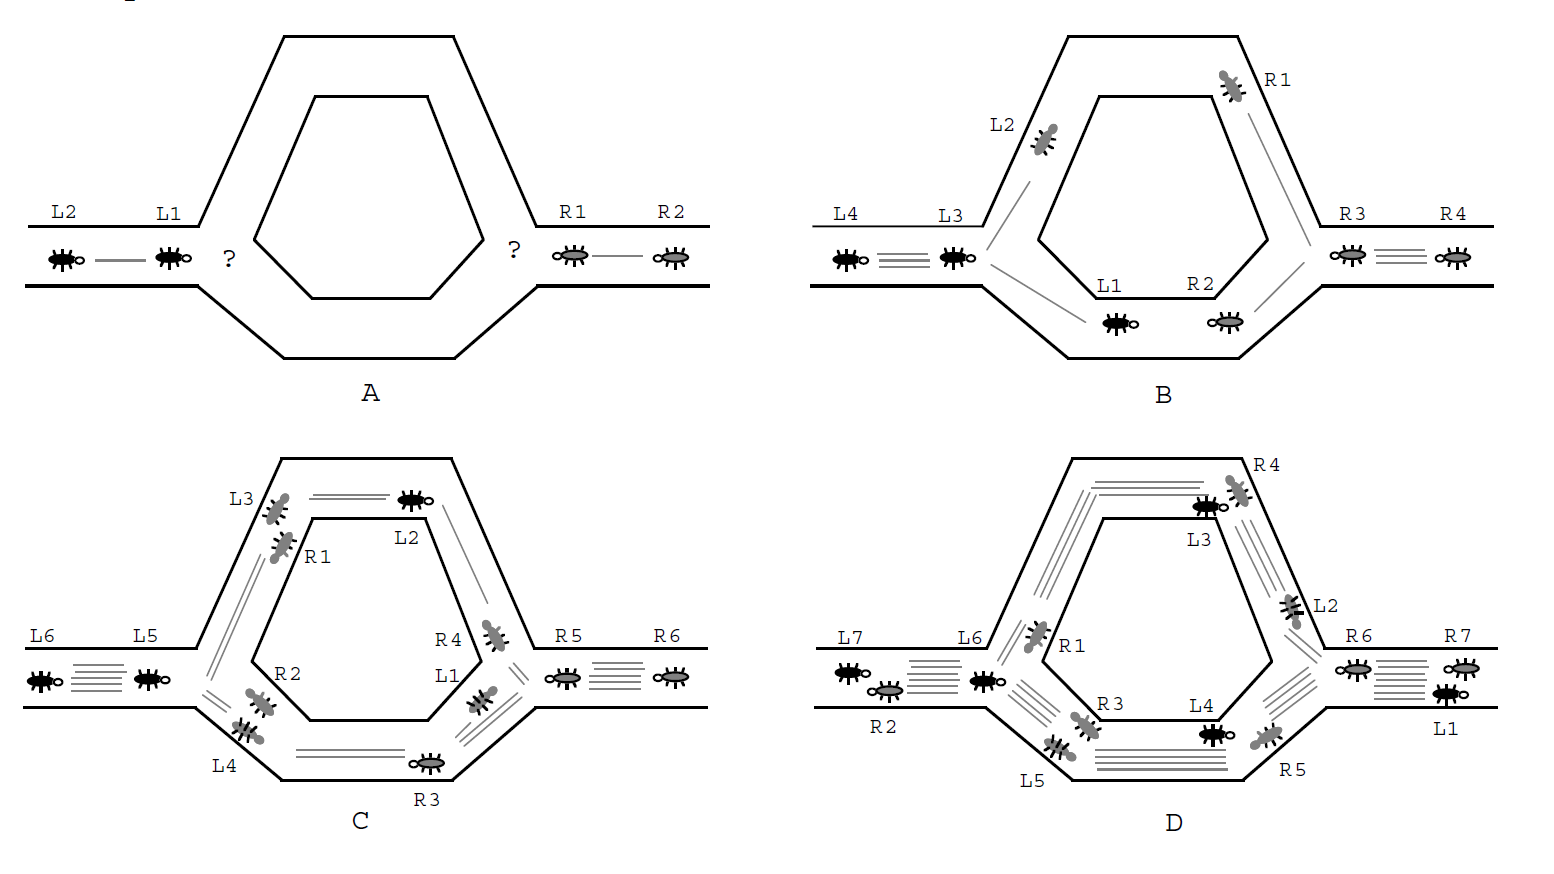
\includegraphics[width=.75\columnwidth]{ants_example}
	\caption{How real ants find a shortest path [Dorigo, Gambardella, et al.].}
\end{figure}
\end{frame}


\begin{frame} \frametitle{Transition rules} 

\begin{block}{Ant Colony Optimization}
\begin{equation*}
P_{ij}^{k} = \frac{\tau_{ij}^{\alpha}~\eta_{ij}^{\beta}}{\sum_{l\in\Psi}\tau_{il}^{\alpha}~\eta_{il}^{\beta}}
\end{equation*}	
\end{block}

\begin{block}{Ant Colony System}
Pseudo random proportional rule:
\begin{equation*}
j = 
\begin{cases} 
\displaystyle\operatorname*{arg\,max}_{j\in J(i)} \{ {[\tau_{ij}]\cdot[\eta_{ij}]^{\beta}} \} & \text{if } q\leq q_0 \quad\quad \text{(exploitation)} \\
S & otherwise \quad \text{(biased exploration)}
\end{cases}
\end{equation*}
where $S$ is a random variable selected according to $P_{ij}^{k}$ 
\end{block}

\end{frame}



\begin{frame} \frametitle{Update rules} 

\begin{block}{Global update rule}
\begin{equation*}
\tau_{ij} \leftarrow (1 - \alpha)\cdot\tau_{ij}~+~\alpha\cdot\tau_{ij}^{k}
\end{equation*}

\begin{equation*}
\Delta\tau_{ij}^{k} = 
\begin{cases} 
1/L_{gb} & \text{if arc}~(i,j)\in~\text{global-best-tour} \\
0		 & \text{Otherwise}
\end{cases}
\end{equation*}

\end{block}

\begin{block}{Local update rule}

\begin{equation*}
\tau_{ij} \leftarrow (1 - \rho)\cdot\tau_{ij}~+~\rho\cdot\tau_{ij}^{k}
\end{equation*}

\begin{equation*}
\Delta\tau_{ij}^{k} = 
\begin{cases} 
1/L_{init} 	& \text{if arc}~(i,j)\in~\text{initial-tour} \\
0    		& \text{Otherwise}
\end{cases}
\end{equation*}
\end{block}

\end{frame}


\begin{frame} \frametitle{Solution encoding} 

\begin{block}{Machine assignment}
\begin{equation} \label{eq:stage1} \tag{stage 1}
S_1 =[~3~2~3~1~4~3~4~2~1~4]
\end{equation}
(interpretation) machine three ($m_3$) has assigned jobs 1, 3 and 6
\end{block}

\begin{block}{Jobs sequencing}
\begin{equation}\label{eq:stage2} \tag{stage 2}
S_2 =
\begin{bmatrix}
9  &  4  &  0 &  0 &  0 &  0 &  0 &  0 &  0 &  0 \\
8  &  2  &  0 &  0 &  0 &  0 &  0 &  0 &  0 &  0 \\
6  &  3  &  1 &  0 &  0 &  0 &  0 &  0 &  0 &  0 \\
5  & 10  &  7 &  0 &  0 &  0 &  0 &  0 &  0 &  0 
\end{bmatrix}
\end{equation}	
(interpretation) machine one ($m_1$) will process jobs in the following order: $9 \rightarrow 4$
\end{block}

\end{frame}


\begin{frame} \frametitle{Transition definition (Stage 1)} 

\begin{block} {Transition rule}
\begin{equation}\label{eq:acsTauStage1} 
j = 
\begin{cases} 
\displaystyle\operatorname*{arg\,max}_{j\in J(i)} \{ {[\tau_{jk}^{I}]\cdot[\eta_{jk}^{I}]^{\beta}} \} & \text{if } q\leq q_0 \quad\quad \text{(exploitation)} \\
S & otherwise \quad \text{(biased exploration)}
\end{cases}
\end{equation}
\end{block}

\begin{block}{Visibility metric}
\begin{columns}[c]
	\begin{column}[c]{6cm}
	\begin{equation} \label{eq:acsEta1Stage1}
	\eta_{jk}^{I} = \frac{1}{P_{jk}}
	\end{equation}	
	\end{column}
	\pause
	\begin{column}[c]{6cm}
	\begin{equation} \label{eq:acsEta2Stage1}
	\eta_{jk}^{I} = \frac{1}{
		\left[ \frac{P_{jk}}{\operatorname*{max}_{m\in M_{j}}(P_{jm})} +
		\frac{E_{jk}}{\operatorname*{max}_{m\in M_{j}}(E_{jm})}\right]}
	\end{equation}
	[Tonelli, Salido, et al. 2016]
	\end{column}
\end{columns}
\end{block}

\end{frame}


\begin{frame} \frametitle{Transition definition (Stage 2)} 

\begin{block} {Transition rule}
\begin{equation} \label{eq:acsTauStage2}
j = 
\begin{cases} 
\displaystyle\operatorname*{arg\,max}_{j\in J(i)} \{ {[\tau_{ij}^{II,k}]\cdot[\eta_{ij}^{II,k}]^{\beta}} \} & \text{if } q\leq q_0 \quad\quad \text{(exploitation)} \\
S & otherwise \quad \text{(biased exploration)}
\end{cases}
\end{equation}
\end{block}

\begin{block}{Visibility metric}
	\begin{columns}[c]
		\begin{column}[c]{6cm}
		\begin{equation} \label{eq:acsEta1Stage2}
		\eta_{ij}^{II,k} = \frac{1}{s_{ijk}}
		\end{equation}
		\end{column}
		\pause
		\begin{column}[c]{6cm}
		\begin{equation} \label{eq:acsEta2Stage2}
		\eta_{ij}^{II,k} = \frac{1}{
			\left[ \frac{s_{ijk}}{\operatorname*{max}_{j'\in J_{k}}(s_{ij'k})} +
			\frac{r_{j}}{\operatorname*{max}_{j'\in J_{k}}(r_{j'})}\right]}
		\end{equation}
		\end{column}
	\end{columns}
\end{block}

\end{frame}


\begin{frame} \frametitle{Pheromone global update} 

\begin{block} {Stage 1}
\begin{equation} \label{eq:acsTauStage1UpdateGlobal}
\tau_{jk}^{I} \leftarrow (1 - \alpha)\cdot\tau_{jk}^{I} +\alpha\cdot\Delta\tau_{jk}^{I,Best}
\end{equation}

\begin{equation}
\Delta\tau_{jk}^{I,Best} = 
\begin{cases} 
1/F(s_{gb}) & \text{if arc}~(j,k)\in~\text{global-best-schedule} \\
0			& \text{Otherwise}
\end{cases}
\end{equation}

\end{block}

\begin{block}{Stage 2}

\begin{equation} \label{eq:acsTauStage2UpdateGlobal}
\tau_{ij}^{II,k} \leftarrow (1 - \alpha)\cdot\tau_{ij}^{II,k} +\alpha\cdot\Delta\tau_{ij}^{II,Best}
\end{equation}
\begin{equation}
\Delta\tau_{ij}^{II,Best} = 
\begin{cases} 
1/F(s_{gb}) & \text{if arc}~(i,j,k)\in~\text{global-best-schedule} \\
0			& \text{Otherwise}
\end{cases}
\end{equation}
\end{block}


\end{frame}


\begin{frame} \frametitle{Pheromone local update} 

\begin{block} {Stage 1}
\begin{equation} \label{eq:acsTauStage1UpdateLocal}
\tau_{jk}^{I} \leftarrow (1 - \rho)\cdot\tau_{jk}^{I} +\rho\cdot\Delta\tau_{jk}^{I,Best}
\end{equation}

	
\begin{equation}
\Delta\tau_{jk}^{I,Best} = 
\begin{cases} 
1/F(s_{init}) & \text{if arc}~(j,k)\in~\text{initial-best-schedule} \\
0			& \text{Otherwise}
\end{cases}
\end{equation}

	
\end{block}

\begin{block}{Stage 2}
	
\begin{equation} \label{eq:acsTauStage2UpdateLocal}
\tau_{ij}^{II,k} \leftarrow (1 - \rho)\cdot\tau_{ij}^{II,k} +\rho\cdot\Delta\tau_{ij}^{II,Best}
\end{equation}

\begin{equation}
\Delta\tau_{ij}^{II,Best} = 
\begin{cases} 
1/F(s_{init}) & \text{if arc}~(i,j,k)\in~\text{initial-best-schedule} \\
0			& \text{Otherwise}
\end{cases}
\end{equation}


\end{block}


\end{frame}


%\subsection{Local Search}

\begin{frame}[fragile] \frametitle{Local search procedure} 


\begin{algorithm}[H]
	\footnotesize
	\caption{Local search procedure}
	\label{alg:acoLocalSearch}
	Set $LocalIteration = 1$\;
	\While{$LocalIteration \leq MaxLocalterations$}{
		Generate random variable ($rv$) from $U(0,1)$\;
		\eIf{$rv < 0.5$}{
			generate neighboring solution for $S_1(Ant)$: $N_1(Ant) \wedge x = 1$\;
		}{
			generate neighboring solution for $S_2(Ant)$: $N_2(Ant) \wedge x = 2$
		}
		Determine $F(N_x(Ant))$\;
		\If{$F(N_x(Ant)) \leq F(Ant)$}{
			$S_x \leftarrow N_x(Ant)$\;
		}
		$LocalIteration = LocalIteration + 1$
	}
\end{algorithm}

\end{frame}


%\subsection{ACS workflow}

\begin{frame}[fragile] \frametitle{Ant colony system workflow} 

\begin{algorithm}[H]
	\footnotesize
	\caption{ACS workflow}
	\label{alg:acoWorkflow}
	Populate the paths with specified pheromone amounts $(\tau_{jk}^{I},\tau_{ij}^{II,k})$\;
	\While{$not~StopCriteria$}{
		Set $Step = 1$\;
		\While{$Step \leq MaxSteps$}{
			\For{$Ant \in Ants$}{
				Solve $Step$ for Stage 1 (Assignment): find $S_1$ according to \cref{eq:acsTauStage1,eq:acsEta1Stage1,eq:acsEta2Stage1}\;
				Solve $Step$ for Stage 2 (Sequencing): find $S_2$ according to \cref{eq:acsTauStage2,eq:acsEta1Stage2,eq:acsEta2Stage2}\;		
			}	
			Update pheromone amounts locally according to \cref{eq:acsTauStage1UpdateLocal,eq:acsTauStage2UpdateLocal}\; 
		}
		Calculate $F(Ants)$ that are associated with $S_1$ and $S_2$\;		
		Execute local search procedure for all ants\;
		Update pheromone amounts globally according to \cref{eq:acsTauStage1UpdateGlobal,eq:acsTauStage2UpdateGlobal}\;
	}
\end{algorithm}


\end{frame}
			% Ant colony system
\section{Evaluation} \label{sec:evaluation}

\subsection{Metrics}

\begin{equation}
F_{1-macro} = \frac{1}{|L|} \displaystyle\sum_{l\in L} F_1(y_l, \hat{y}_l)
\end{equation}

\begin{equation}
F_1 = 2 \cdot \frac{precision \cdot recall }{precision + recall}
\end{equation}

\begin{equation}
precision = \frac{1}{|L|} \displaystyle\sum_{l\in L} Pr(y_l, \hat{y}_l)
\end{equation}

\begin{equation}
recall = \frac{1}{|L|} \displaystyle\sum_{l\in L} R(y_l, \hat{y}_l)
\end{equation}


\subsection{Results}

Put an intro over the results that will be analyzed and then comments over them

table of only the 5 models main models and 6 kind of preprocessing
only the mean and say that is 10 fold CV

table of word representation




		% Evaluation
% A chapter named 'Your first document' is created
\chapter{Conclusion} \label{chapter:conclusion}

Here you have only the put all the concept that could be presented in the work and then in the literature review you will illustrate different proposed solution to the exposed topics.		% Conclusions


% The bibliography is printed with \bibliography{}. With the command \bibliographystyle{} a style is picked.
%\bibliographystyle{plain}
%\bibliography{refs/references}


% To close your document, add the \end{document} command. Everything after this command will not be processed.
\end{document}